\section{Taxonomy}
Our taxonomy is a software abstraction hierarchy where `basic programming functionality' such as code compilation and syntax checking is at the least abstract level.
Software architecture analysis and design is at the most abstract level.
As we ascend the levels, just as with Koopman's pyramid in Figure \ref{fig:koopman_pyramid}, software challenges a) rely on successfully solving the challenges below, and b) become more difficult to automate (e.g., crafting design rules vs code smells). 

The challenges further up the hierarchy are nonetheless more important for software quality attributes (QA) \cite{Ernst2017} and for a well-engineered software system.
For example, an automated solution to the top level of the taxonomy would be able to follow heuristics to engineer a well designed software system, one which would be easy to modify and scale to sudden changes in use.

The question remains where we stand today, and where the line (or area) exists between places where the AI can take control, and where a human engineer should be involved, just like the distinction between a self-driving car and one where humans still need to be alert.
Our taxonomy in Figure \ref{fig:levels} captures this as a distinction between what seems automatable or is already automated (green, lower) and levels that are not yet automated (red, higher).
% Syntax reflects syntactically correct code and is detected by the compiler. Standards and warnings include `-w' style compiler flags. Smells are aspects of source code that are sub-optimal by general acceptance; paradigms and idioms are good practices for languages or application styles. Finally, design refers to optimal design approaches for system quality attributes.

\begin{figure}
    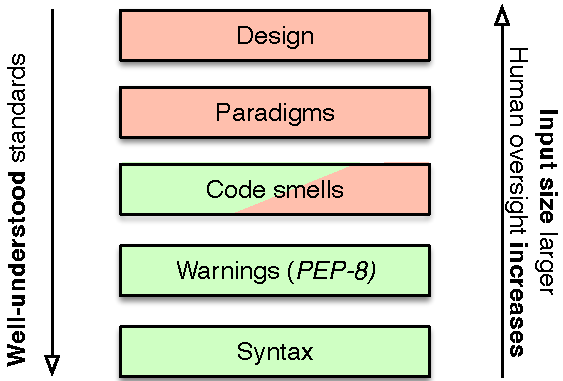
\includegraphics[width=.7\linewidth]{Figures/taxonomy-copilot.pdf}
    \caption{Hierarchy of software abstractions. Levels depend on one another as abstraction increases. Parentheticals are examples of each level. As we move up the hierarchy, we require more human oversight of the AI; as we move down the hierarchy, rules for detecting problems are easier to formulate. Green levels are areas where AI supported programming works reasonably well, while red levels are difficult or impossible, as we show in the paper. }
    \label{fig:levels}
\end{figure}

To motivate this taxonomy, we look at how Copilot, as a representative AI supported programming tool, is able to produce code that aligns with two of the levels in our taxonomy. 
One is the way Copilot manages \emph{language idioms}.
A language idiom~\cite{Alexandru2018} is commonly thought of as the `one way to do it', where `it' might include looping constructs, storing data, or initializing data structures.
The second is the way Copilot is able to \emph{prevent code smells} by suggesting and understanding community-agreed best practices in programming, for example, in conducting code reviews.
% \neil{third? maybe SQ smells design smells.}.
For each level, we compare the recommended \textbf{ideal} solution with the solution Copilot suggests. Since Copilot generates up to 10 suggestions, we also consider where the suggestion appears in the list (if at all). 